\documentclass[11pt]{article}

%opening
\usepackage{caption}
\usepackage{mcexam}
\usepackage{amsmath}
\usepackage{amsfonts}
\usepackage{graphicx}
\usepackage{enumerate}
\usepackage{tikz}
\usepackage{float}
\usepgflibrary{arrows}
\usepackage{todo}
\everymath{\displaystyle}
\pagestyle{empty}
\usepackage{lastpage} % this calculates the page number of the last page
\usepackage{fancyhdr}
\pagestyle{fancy}
\lhead{\textsf{Spring 2016}}
\chead{\textsf{Math 131 -- Midterm Exam 1A}}
\rhead{\textsf{Page \thepage\ of \pageref{LastPage}}}
\cfoot{}
\rfoot{\textsf{\thepage}}

\newcommand{\series}[3]{\displaystyle \sum_{{#1}={#2}}^{#3} }
\newcommand{\limit}[2]{\displaystyle \lim_{{#1} \rightarrow {#2}} }
\newcommand{\din}[2]{\displaystyle \int_{#1}^{#2}}
\newcommand{\Int}{\displaystyle \int}
\newcommand{\Q}{\ensuremath \mathbb{Q}}
\newcommand{\R}{\ensuremath \mathbb{R}}
\newcommand{\C}{\ensuremath \mathbb{C}}
\newcommand{\Z}{\ensuremath \mathbb{Z}}
\newcommand{\N}{\ensuremath \mathbb{N}}
\newcommand{\isom}{\ensuremath \cong}
\newcommand{\inv}{\ensuremath ^{-1}}
\newcommand{\ot}{\ensuremath \otimes}
\newcommand{\op}{\ensuremath \oplus}

\Course{Math 131}{Principles of Calculus}
%\Instructor{Steven McKay}
\TestName{Exam 1A\hfill{\bfseries\Huge RED}}
\Date{}
%\Section{}


\begin{document}
\Head
\begin{instructions}
\item For questions which require a written answer, show all your work.  Full credit will be given only if the necessary work is shown justifying your answer.
\item Simplify your answers.
\item Calculators are allowed.
\item Should you have need for more space than is allocated to answer a question, use the back of the exam.
\item Please do not talk about the test with other students until exams are handed back.
\end{instructions}
\PointTable{2}
%\hrule width \linewidth height 2pt\vspace{2pt}%
%\hrule width \linewidth height 1pt\vspace{2pt}%
%\hrule width \linewidth height 1pt%
%\vspace{4mm}%
%\noindent {\bf For Instructor use only.}\\ \vspace{-.2in}%
%\begin{center}
%{\Large
%\begin{tabular}{|p{0.75in}|p{0.4in}|p{0.4in}|p{0.4in}|p{0.4in}|p{0.4in}|p{0.4in}|p{0.4in}|p{0.4in}|p{0.4in}|}
%\hline
%Question&MC&11&12&13&14&15&16&17&Total\\\hline
%Points&30&10&10&10&10&10&10&10&100\\\hline
%Earned&&&&&&&&&\\\hline
%\end{tabular}
%}
%\end{center}
\nextpage

\vspace{.2in}

\noindent \emph{{\bf Part I: Multiple Choice (5 points each)} Mark the correct
answer on the bubble sheet.}
For questions 1-4, use the following graph of $f(x)$:\\


\begin{minipage}{\linewidth}% to keep image and caption on one page
\centering
\makebox[\linewidth]{}
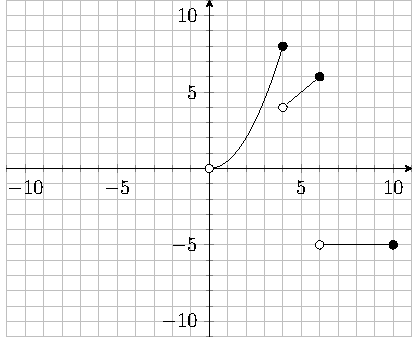
\includegraphics{exam1graph1.pdf}
\captionof{figure}{$f(x)$}\label{graph1exam1}%      only if needed  
\end{minipage}


\begin{questions}
\begin{multiplechoice}{5}
%8.5,8.6

\question According to the graph of $f(x)$, the $\lim_{x\to 4^+}f(x) $ equals which of the following.
\begin{answers}{3}
\ans $8$
\ans $4$
\ans $0$
\ans $-3$
\ans The limit does not exist.
\end{answers}

%\textbf{Solution: d}


\question According to the graph of $f(x)$, the $\lim_{x\to 10^-}f(x) $ equals which of the following.
\begin{answers}{3}
\ans $+\infty$
\ans $0$
\ans $-2$
\ans $-5$
\ans The limit does not exist.
\end{answers}

%\textbf{Solution: a}\\

\question According to the graph of $f(x)$, the $\lim_{x\to 2}f(x) $ equals which of the following.
\begin{answers}{3}
\ans $2$
\ans $0$
\ans $-3$
\ans $-4$
\ans The limit does not exist.
\end{answers}

%\textbf{Solution: b}\\




\question According to the graph of $f(x)$, the function $f(x)$ is not continuous at $x=6$ because
\begin{answers}{3}
\ans $f(x)$ is not defined at $x=6$.
\ans $\lim_{x\to 6}f(x) \neq f(6)$.
\ans $\lim_{x\to 6}f(x)$ does not exist.
\ans there is a horizontal asymptote at $x=6$. 
\ans there is a vertical asymptote at $x=6$.
\end{answers}

%\textbf{Solution: e}

%11.1,2

\nextpage

\question The graph of $g(x)$ is given below.\\

\begin{minipage}{\linewidth}% to keep image and caption on one page
\centering
\makebox[\linewidth]{}
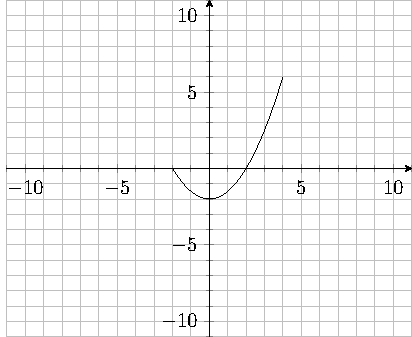
\includegraphics{exam1graph2.pdf}
\captionof{figure}{$g(x)$}\label{graph2exam1}%      only if needed  
\end{minipage}
According to the graph above, the domain and range of $g(x)$ are
\begin{answers}{2}
\ans Domain: $[-2,6]$, Range: $[-4,2]$
\ans Domain: $[-2,4]$, Range: $[-2,6]$
\ans Domain: $[-6,8]$, Range: $[-2,6]$
\ans Domain: $[-12,12]$, Range: $[-8,8]$
\ans Domain: $[-2,-6]$, Range: $[-2,4]$
\end{answers}
% Answer: 232/99

\question Find the domain of $f(x) = \frac{x}{x^2-4}$.
\begin{answers}{2}
\ans $(-2,2) \cup (2, \infty)$
\ans $(-\infty, -4) \cup (-4,4) \cup (4, \infty) $
\ans  $(-\infty, -4) \cup (0, \infty)$
\ans  $(-\infty, -2) \cup (-2,2) \cup (2, \infty)$
\ans $[-2,2)$
\end{answers}


\question Let $f(x) = \sqrt{9-x^2}$ and $g(x)=\sqrt{1+x}$.  What is the domain of $f(x)+g(x)$?
\begin{answers}{2}
\ans $[-3,3]$
\ans $[-1,3]$
\ans $[-3,\infty]$
\ans $[-1,\infty]$
\ans $[-3,1]$
\end{answers}

\nextpage

\question Given a function $f(x)$, then the graph of $-f\left(\frac{x-4}{4}\right)$ will be
\begin{answers}{2}
\ans the graph of $f(x)$ shrunk horizontally by a factor of 4, shifted 4 units up and reflected horizontally.
\ans the graph of $f(x)$ stretched vertically by a factor of 4, shifted 4 units up and reflected horizontally.
\ans the graph of $f(x)$ stretched vertically by a factor of 4, shifted 4 units to the right and reflected vertically.
\ans the graph of $f(x)$ stretched horizontally by a factor of 4, shifted 4 units to the left and reflected vertically. % 
\ans the graph of $f(x)$ shrunk horizontally by a factor of 4, shifted 4 units to the right, and reflected vertically.
\end{answers}


\question Jane notices that football game attendance is higher when the weather is warmer.  She finds that 90,000 fans attended a game when the temperature was $75^\circ$ F and that 60,000 fans attended when the temperature was $45^\circ$ F.  Make a linear model that describes Jane's findings, where $t$ is the temperature in degrees Fahrenheit and $F(t)$ is the number of fans attending a game.
\begin{answers}{3}
\ans $F(t) = 1000t+15,000$
\ans $F(t) = 1000t-30,000$
\ans $F(t) = 500t+40,000$
\ans $F(t) = 500t - 60,000$
\ans none of these
\end{answers}

\question 500 years ago, a radioactive sample had mass 100mg.  At present, the sample has mass 80mg.  Assuming the sample decays exponentially, how much mass will it have in 800 years?
\begin{answers}{2}
\ans 50 mg
\ans 55.98 mg %
\ans 65.49 mg
\ans 62.21 mg
\ans 69.98 mg
\end{answers}


\end{multiplechoice}
\vspace{.2in}

\nextpage
\noindent \emph{{\bf Part II: Free Response}{  Show all work}}
\question[12] Let $f(x)=x^2-4$ and $g(x) = x+2$.\\

a.) (5 points) Calculate the domain of $\frac{g(x)}{f(x)}$.
\vspace{1.25in}

b.) (7 points) Calculate and simplify $h(x) = \frac{f(g(x))-f(2)}{x}$.
\vspace{2.25in}




\question[10] Evaluate the limit algebraically (show all your work!)
\[\lim_{x\to 12} \frac{\sqrt{x^2+25} - 169}{x-12}.\]
\vspace{3.25in}

\question[8] For the function 
\[f(x) = \frac{x^2-4x+3}{x^2+3x+2},\]
a.) (4 points) Find the vertical asymptotes of $f(x)$.
\vspace{2.25in}

b.) (4 points) Find the limit $\lim_{x\to \infty} f(x)$.
\vspace{2.25in}

\question[15] Evaluate each limit as a number, $\infty$, or $-\infty$.

a) (3 points) $\displaystyle \lim_{x\to\infty} \frac{6x^5 + 3x^2}{2x^5 - 3x}$

\vspace{1.25in}

b) (3 points)  $\displaystyle \lim_{x\to\infty} \frac{3x^4 - 2x^2}{x^3 +1}$

\vspace{1.25in}

c)  (3 points)  $\displaystyle \lim_{x\to-\infty} \frac{3x^4 - 2x^2}{x^5 +2}$

\vspace{1.25in}

d) (3 points) $\displaystyle \lim_{x\to-\infty} \frac{7e^x - x^2}{9e^x -x^7}$

\vspace{1.25in}

e)  (3 points) $\displaystyle \lim_{x\to-\infty} \frac{x^3 - x^2}{2x^3 -x}$

\vspace{1.25in}


\question[10] Find $f\inv(x)$ for the following function,
\[f(x) = \frac{e^{2x+2}}{e^{x-1}} - 3.\]

\vspace{3.25in}


\question[15] Katie believes that football teams that throw long passes tend to perform better.  She collects data on five football teams describing the longest pass the team throws during the season and the average number of points their football teams scored in a season.  \\
\begin{center}
  \begin{tabular}{| c | c |}
    \hline
    Longest Pass (yds) & Average Points \\ \hline \hline
    25 & 8.9  \\ \hline
    35 & 11.4  \\ \hline
    55 & 26.2  \\ \hline
    60 & 26.7  \\ \hline
    70 & 32.8  \\ \hline
  \end{tabular}
\end{center}

a.) (3 points) Find a linear model for this data set by \textbf{using the first and last points} in the table.
\vspace{1.5in}

b.) (5 points) Find a better linear model by computing the linear regression of all 6 data points.
\vspace{1in}


c.) (3 points)   Use the linear regression to predict the average number of points a team would score whose longest pass is 50 yards.
\vspace{1in}


d.) (4 points) Use the linear regression to predict the average number of points a team would score whose longest pass is 5 yards.  Is this a realistic prediction?  Why or why not?
\vspace{1in}

%\begin{minipage}{\linewidth}% to keep image and caption on one page
%\makebox[\linewidth]{}
%\begin{center}
%\includegraphics{exam1graph3.pdf}
%\end{center}
%\captionof{figure}{Average Points per Game}\label{graph3exam1}%      only if needed  
%\end{minipage}




\mbox{}
\end{questions}
\end{document}

*************************************************************************
*************************************************************************
